\chapter{Literature Review}
\label{ch:Literature Review}


\section{Inverter-Based Resources (IBR): GFL vs GFM}

As a result of the increasing demand in power systems for renewable energy technologies, inverter-based resources (IBRs) are becoming a relevant component of AC power systems. Typically, Distributed Energy Resources (DERs) produce electricity as Direct Current (DC); therefore, an inverter is required to transform the waveform into Alternating Current (AC). The inverter thus acts as the interface between DERs and the electric grid.

Due to the natural intermittency of renewable energies such as wind and solar, extracting the maximum available energy at any time has been a major objective in the integration of these assets. However, these assets are not able to provide inertia, unlike the large rotating masses of synchronous generators. Consequently, the reduction in mechanical inertia from synchronous machines has become a topic of concern for grid operators. This reduction results in larger frequency swings when the system experiences disturbances, such as load variations. These events can consequently trip loads or inverter-based units, thereby increasing reliability issues for the power system \cite{8586162}

The primary objective of IBRs is to supply active and reactive power to the grid; however, depending on their interaction with the grid, their behavior under disturbances, and the controller implementation, IBRs can be classified into two major groups: grid-following (GFL) and grid-forming (GFM) inverters.\cite{Rathnayake2021}

From an economic point of view, it is generally more attractive to install GFL inverters, since the main goal is to sell as much available energy as possible to the grid. GFL inverters can maximize energy production through algorithms such as Maximum Power Point Tracking (MPPT). Nevertheless, as the share of this type of inverter increases within the power system, voltage and frequency regulation become a challenge. To address this, grid operators have imposed requirements for inverters to support the grid by injecting reactive power and by adjusting their active power output in response to grid variations.

As an illustrative example, \cite{Mirafzal2020} discusses reactive power (Q) support. Whenever a voltage deviation occurs, the IBR should be able to detect and respond accordingly. In the case of a voltage decrease, the inverter must supply reactive power according to a predefined droop setting; conversely, for a voltage increase, the inverter should absorb (supply negative) reactive power.

As previously discussed, the main function of a Grid-Following (GFL) inverter is to inject active and reactive power into the grid. The distinction between GFL and Grid-Forming (GFM) inverters lies not only in the manner in which these inverters deliver active and reactive power (P,Q), but also in their fundamental control objectives. While GFL inverters rely on the existing grid to define voltage and frequency, GFM inverters actively regulate these parameters, establishing and maintaining the grid’s voltage and frequency reference.

The main distinction between Grid-Following (GFL) and Grid-Forming (GFM) inverters lies in their underlying control principles and the way they interact with the grid.

Overall, both GFM and GFL inverters share similar grid-support and power-generation objectives during grid-connected operation. These objectives are achieved either through active and reactive power adjustments in the case of GFL control, or through voltage and frequency regulation in the case of GFM control \cite{9751441}

\subsection{Grid Following Inverters}

A fundamental challenge in low-inertia power systems is that most existing inverter controllers are equipped with GFL control. 
This type of control is designed under the assumption that inertial sources, such as synchronous generators or grid-forming inverters, regulate the voltage and frequency of the grid. \cite{osti_1813971}. Another challenge arises because large PV plants or onshore wind farms are often located far from consumption centers; consequently, long transmission lines are required. As a result, the grid impedance “seen” from the IBR side tends to be high, and such areas are commonly referred to as weak parts of the grid. In these sections, maintaining voltage regulation through conventional methods becomes difficult.

Currently, the majority of PV inverters connected to the grid operate as grid-following (GFL) inverters. This type of inverter adjusts its power output by synchronizing with the grid through a Phase-Locked Loop (PLL). The PLL works by continuously measuring the angle and frequency of the grid voltage. \cite{8586162}. 

The synchronization of a GFL inverter is achieved through a Phase-Locked Loop (PLL). In this configuration, the inverter behaves as a current source, injecting current into the existing grid voltage. From a control perspective, a GFL inverter can be modeled as a controlled current source connected in parallel with a high impedance. The inverter measures the voltage at the Point of Common Coupling (PCC), $v_{PCC} $ , using the PLL. This signal is  then transformed via the Clarke and Park Transformation into the direct and quadrature (dq) components. The power control sets the desired dq currents required to inject the desired Active and Reactive Power. The Current Control source model is shown in Fig 2.1. $C_{p}$ denotes the outer power control loop and $\theta$ represents the phase angle. Under the GFL operation, only
current magnitude and phase angle in the output current are adjusted to achieve the desired active/reactive power outputs. The current source frequency remains identical to the grid frequency.

\begin{figure}[htbp!]
 \centering
 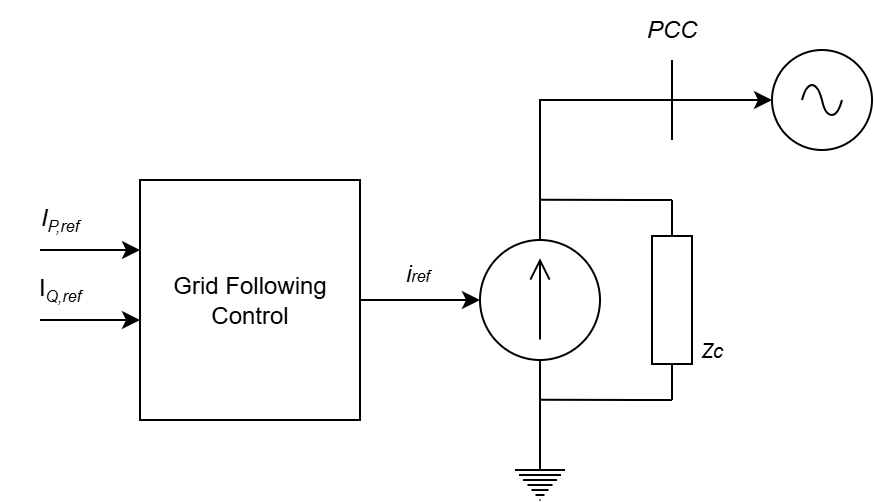
\includegraphics[width=0.8\textwidth]{Figures/Chapter 2/GFL Control Structure.png}
 \caption{fig:Grid Following Inverter Control Structure \cite{11041180}}
 \label{fig:GFL Current Control Source Approximation}
\end{figure}

The Grid-Following (GFL) control strategy operates by delivering the commanded active $P_{ref}$ and reactive $Q_{ref}$ power based on the grid measurements provided by the PLL. 
The power control block calculates the reference currents, which are expressed in the dq-frame and regulated by a fast inner current-control loop that ensures the inverter output current follows its reference accurately. 
In this way, the inverter can be represented as a controlled current source connected to the grid at the PCC through the grid impedance, depending on the existing grid voltage to maintain synchronization and power delivery.  
During large disturbances, the GFL inverter detects changes through voltage and current measurements, which inherently introduce delays in the provision of active and reactive power support. 
From a small-signal stability perspective, since the GFL inverter relies on the PLL for grid voltage and angle measurements, its stability margin can be significantly reduced under sudden grid variations.\cite{Rathnayake2021}

Next, the detailed control blocks of the Grid-Following Inverter is presented. The measured grid current is denoted by $I(f)$
The inverter output voltage is represented by $U_{out}$, and $\theta$ denotes the phase angle of the grid voltage. After the inverter is synchoniyed within the grid, the control references are then sent to the control blocks to achieve the desired performance. The GFL inverter, aside from its capability to provide limited grid support, is primarily designed for efficient power conversion, enabling it to deliver high-quality power to the grid under normal grid operating conditions. Beyond these limits, the GFL inverter must be disconnected. \cite{9751441}

\begin{figure}[htbp!]
 \centering
 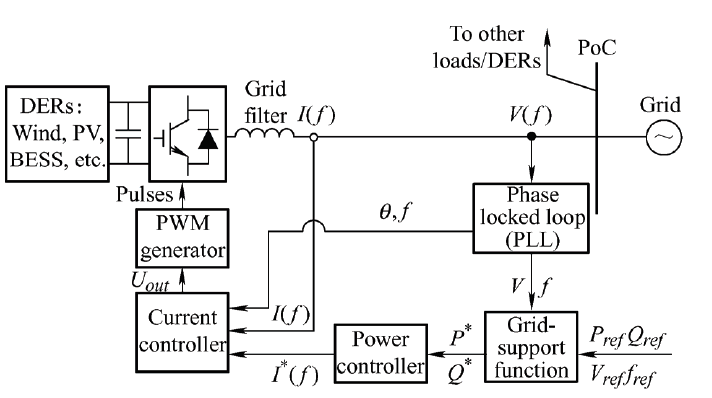
\includegraphics[width=0.8\textwidth]{Figures/Chapter 2/GFL Detailed Control Block.png}
 \caption{fig:Grid Following Inverter Detailes Control Blocks \cite{9751441}}
 \label{fig:Grid Following Inverter Detailes Control Blocks}
\end{figure}




\subsection{Grid Forming Inverters}

In order to address the challenge of a high increase of Grid Following Inverters (GFL), the Grid Forming Control was introduced, the need for one or multiple inverters that is able to operate as voltage and/or frequency regulator(s) to form a local power grid was then presented. 
GFM control do not depend on a PLL, since they are able to self-synchronize with the grid, they are able to create its own voltage and frequency reference. \cite{10968238}
As mentioned before, GFL inverters rely on PLLs to synchronize with an existing grid. In contrast, GFM can autonomously create or establish voltage and frequency references, this capability allows them to improve stability and support capabilities for the grid. \cite{11041180}

Grid-Forming (GFM) converters operate as voltage sources that self-synchronize by internally generating their own voltage and frequency references. By emulating the inertia and damping characteristics of synchronous machines, GFM controllers provide enhanced frequency and voltage support. 
These capabilities make them particularly robust in weak-grid, islanded, or high-renewable environments, where fast and adaptive control is crucial. Overall, GFM converters exhibit higher independence, stability, and flexibility under varying grid conditions, 
positioning them as a key enabling technology for future power systems with high shares of renewable energy. \cite{11041180}

\begin{figure}[htbp!]
 \centering
 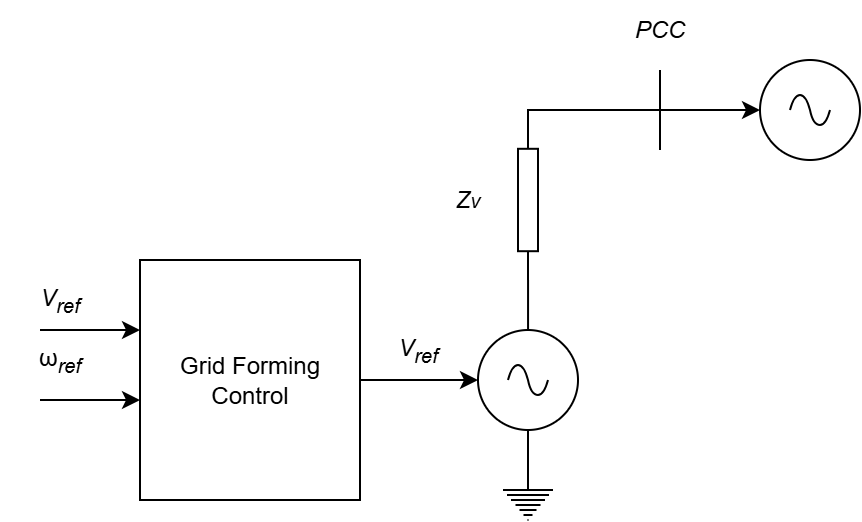
\includegraphics[width=0.8\textwidth]{Figures/Chapter 2/GFM Control Structure.png}
 \caption{fig:Grid Forming Inverter Control Structure \cite{11041180}}
 \label{fig:GFM Control Structure}
\end{figure}
In this case $Z_{load}$ corresponds to the sum of all other loads in the network during islanding operations.
\begin{figure}[htbp!]
 \centering
 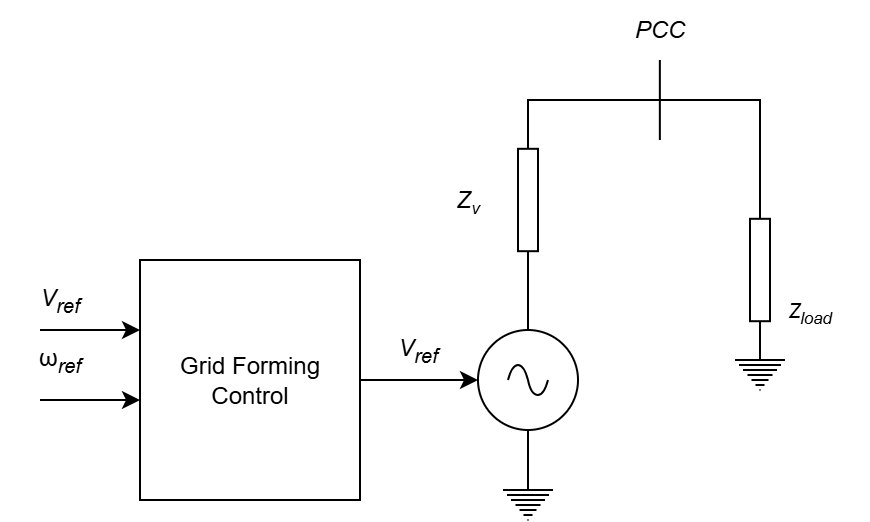
\includegraphics[width=0.8\textwidth]{Figures/Chapter 2/GFM Control Structure Islanding Operation.png}
 \caption{fig:Grid Forming Inverter Control Structure Islanding Operation \cite{9751441}}
 \label{fig:GFM Control Structure Islanding Operation}
\end{figure}

Among the most widely implemented control strategies for Grid-Forming (GFM) inverters are the droop control, virtual oscillator control (VOC), and virtual synchronous generator (VSG) approaches. These methods enable GFM inverters to provide voltage, frequency, and inertia support to the power grid, while ensuring stable and coordinated operation under parallel inverter conditions. Moreover, additional functionalities have been incorporated into GFM inverters, such as self-synchronization — specifically proposed for two-stage inverter architectures — which introduces DC-link voltage regulation through droop control. Other features include the seamless mode transition function, which enables flexible operation of a microgrid between grid-connected and islanded modes; the black-start capability, allowing system restoration after a complete blackout; and the coordinated control function, which facilitates inverter operation under unbalanced grid conditions. \cite{9751441}.

Next, the detailed control blocks for the GFM are presented. In contrast to the GFL inverter, the GFM does not necessarily require synchronization. Under normal grid-connected operation, the GFM can follow power reference signals provided by a system-level controller or an MPPT algorithm, with the purpose of delivering high-quality power to the grid. Conversely, during abnormal grid conditions, the GFM is capable of generating its own voltage and frequency based on the preset reference values of the controller, without the need for a PLL.GFM allows providing direct voltage, frequency and inertia support to the utility grid. \cite{9751441}


\begin{figure}[htbp!]
 \centering
 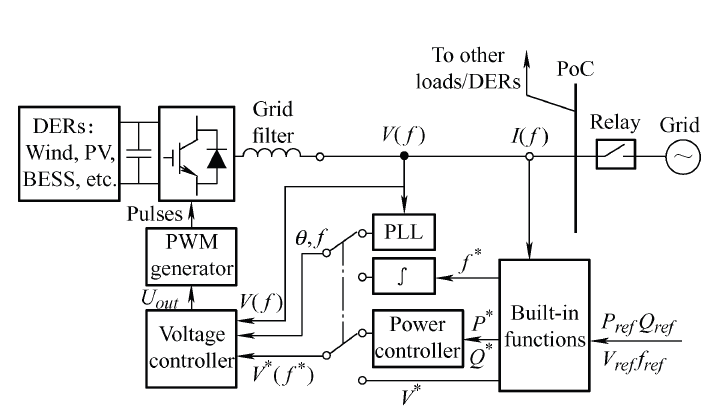
\includegraphics[width=0.8\textwidth]{Figures/Chapter 2/GFM Detailed Control Block.png}
 \caption{fig:Grid Forming Inverter Detailed Control Blocks \cite{9751441}}
 \label{fig:Grid Forming Inverter Detailed Control Blocks}
\end{figure}

\section{GFM Control Methods}

Distributed Generators (DGs) are usually composed of a DC link and two-stages: input-side converter and grid-side converter. The input side varies depending on the specific type of technolgy used and the enregy source used. On the other hand, the grid-side converter is normally a dc/ac converter. 

\section{Power System Stability and Resilience}
\section{Frequency and Voltage Stability Indicators}
\section{Grid Strength and Short-Circuit Ratio}
\section{Real World Examples}
\section{Conventional Stability Support}
\section{Research Gap and Motivation}
\section{German Energy Market}
\section{Grid Stability}
\section{Ancillary Services}


